\documentclass{article}
\usepackage[utf8]{inputenc}
\usepackage{graphicx}
\usepackage{xfrac}
\usepackage{indentfirst}
\usepackage{amsmath}
\usepackage{hyperref}
\hypersetup{
    colorlinks=true,
    urlcolor=blue,
    linkcolor=black
}

\graphicspath{{./img}}

\title{Electrical Components and Circuits Reference}
\author{Marine Maisonneuve, Devaughn Menezes, Andrew Rocco, Eugene Min }
\date{September 2020}


\begin{document}

\maketitle

\tableofcontents

\section{Common Circuit Symbols}

\begin{tabular}{c|c}
    Name & Symbol \\
    \hline
    Ground & 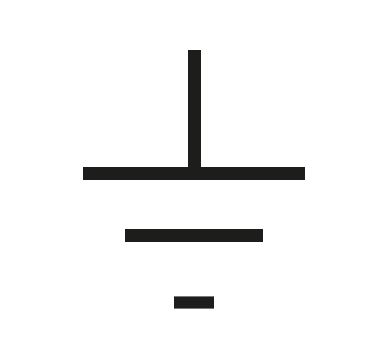
\includegraphics[width=0.08\textwidth]{img/Symbol G7_Earth.JPG}\\
    \hline
    Resistor & 
    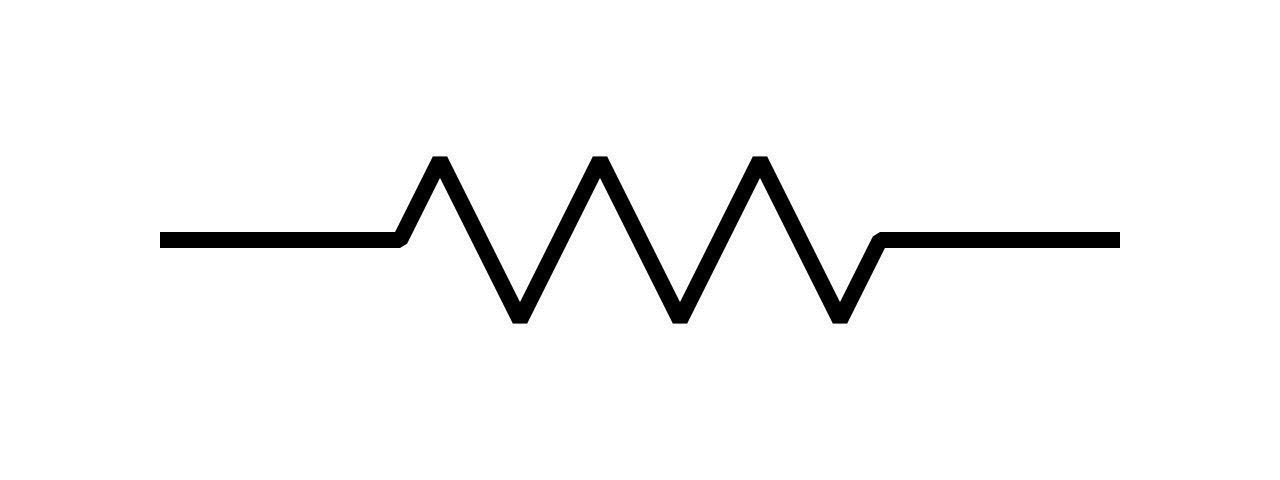
\includegraphics[width=0.2\textwidth]{img/1280px-Resistor_symbol_America.svg.png}\\
    \hline
    Diode & 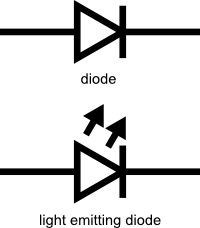
\includegraphics[width=0.2\textwidth]{img/51f1c87ace395fea20000004.png}\\
    \hline
    Capacitor & 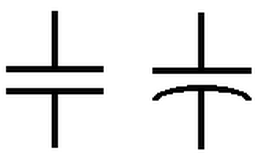
\includegraphics[width=0.2\textwidth]{img/Screenshot_20200913_143337.png} \\
    \hline
    MOSFET & 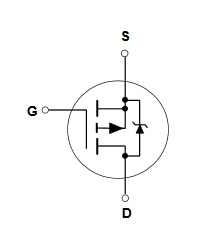
\includegraphics[width=0.2\textwidth]{img/62fe4e5439abf066e1badb3f8a73b483b52614ec.jpeg} \\
    \hline
    Inductor & 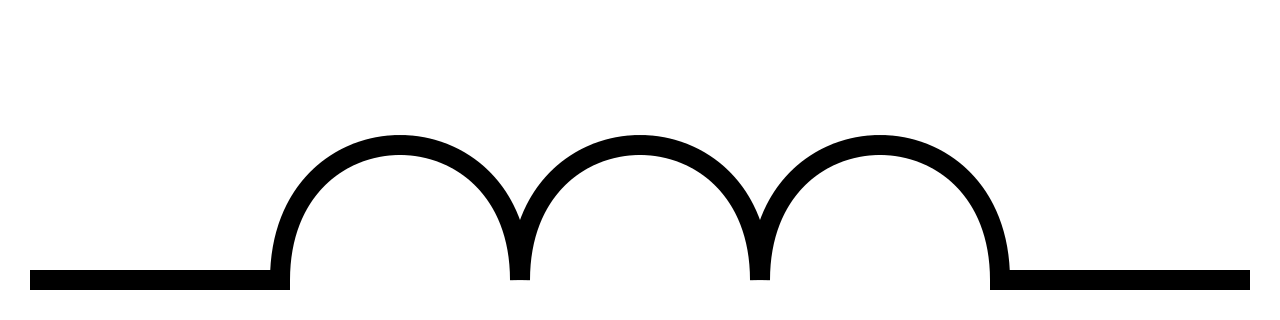
\includegraphics[width=0.2\textwidth]{img/1280px-Inductor_symbol.svg.png}\\
    \hline
    Voltage Source & 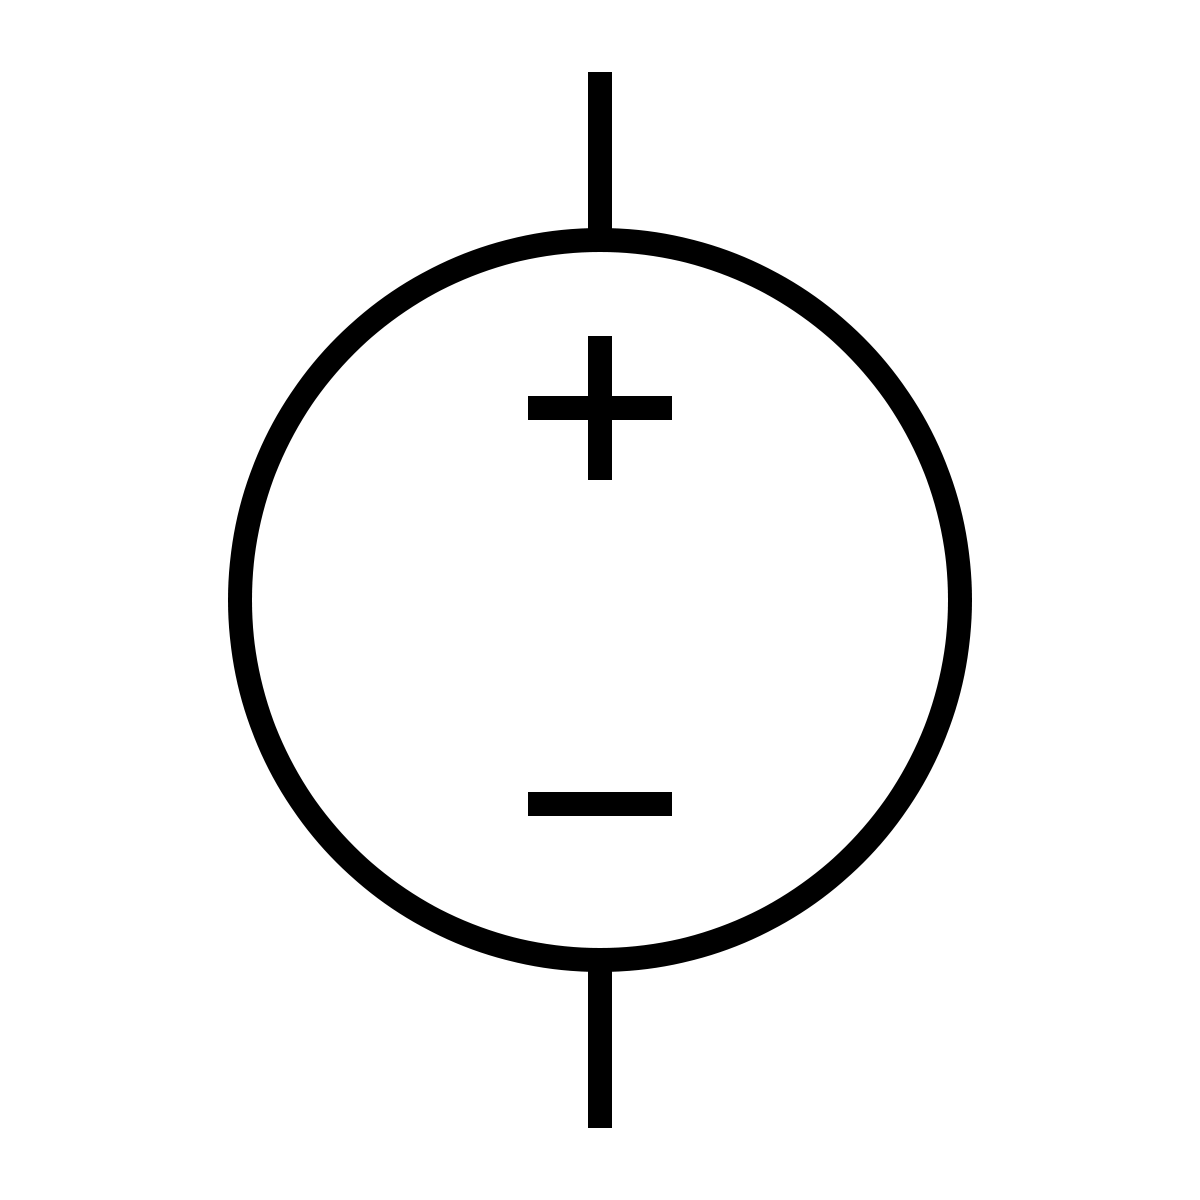
\includegraphics[width=0.12\textwidth]{img/1200px-Voltage_Source.svg.png}
\end{tabular}

\section{Basic Concepts and Definitions}

\begin{tabular}{c|c|c}
    Physical Quantity & Units & Equations \\
    \hline
    Time (t)  & Second & (SI Unit) \\
    Charge (Q) & Coulomb (C) & (SI Unit) \\
    Current (I) & Ampere (A) & $I = \sfrac{Q}{t}$ \\
    Energy (E) & Joule (J) & E = $V \cdot I \cdot t$ \\
    Voltage (V) & Volt (V) & V = $\sfrac{E}{Q}$ \\
    Power (P) & Watt (W) & P = $\sfrac{E}{t} = V \cdot I$ \\
\end{tabular}

\section{Electricity Basics}
Electricity is, as defined by Wikipedia:
\begin{center}
   [A] set of physical phenomena associated with the \textbf{presence} and \textbf{motion} of \textbf{electric charge}.
\end{center}

In other words, a flow of \textbf{electrical charges}.

\subsection{Electric Charge}
In short, particles can be positively or negatively charged. 
\textbf{Electric Charge} is a physical property of particles. On an atomic level, charges carried by \textbf{electrons} are negative and \textbf{protons/nuclei} are positive. Particles with like charges repel each other and particles of opposite charges attract each other.

\subsection{Voltage}
\begin{figure} [h]
    \centering
    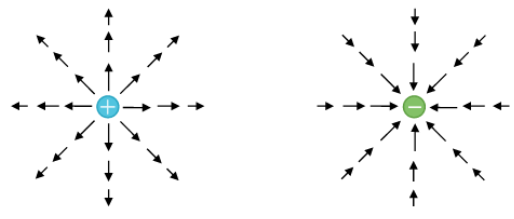
\includegraphics[width=0.7\textwidth]{img/E_Field.png}
    \caption{Charged particles create electric fields}
    \label{fig:E_Field}
\end{figure}
Charged particles create electric fields. If a charge is placed in such a field, there exists a potential difference which causes these particles to move.

\textbf{Voltage} is the driving force for electrical applications. It is an \textbf{electric field potential difference}. Charged particles naturally move from higher potential to lower potential. The amount of energy required to move from this higher potential to a lower potential is described as electrical potential energy. At any point within an electrical field, the amount of electrical potential energy per unit of charge determines the electric potential, measured in Volts (V). The polarity of voltage does not necessarily matter: charges may flow from 5V to 3.3V and also from -5V to -12V. Charged particles always move if there is a potential difference in place. 
\\We can measure electric potential using the following equation:
\begin{center}
Voltage = Electric Potential Energy (in joules)/Charge of Particle (in coulombs)
\end{center}

\begin{figure}
    \centering
    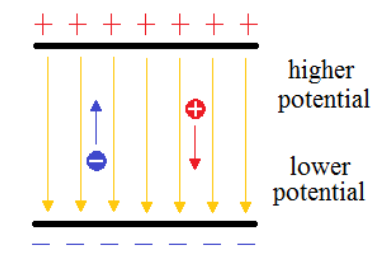
\includegraphics[width=0.7\textwidth]{img/E_Potential.png}
    \caption{Visual of Electric Potential}
    \label{fig:E_Potential}
\end{figure}

\subsection{Current}
Current is induced when charges flow due to an electric potential.

When a potential difference exists in a circuit, charged particles will flow with a certain speed (called drift speed). The \textbf{net flow} of charged particles is called \textbf{current(I)}, measured in \textbf{Amperes (A)}. By convention, the current direction is \textbf{opposite} to the direction of the electron flow. Current is usually induced by voltages, so when there is no voltage, charged particles move randomly so there exists no net flow and thus no current.


\subsection{Resistance}

\textbf{Resistance} is a measure of the \textbf{difficulty for current to pass} through a component, it is measured in Ohms ($\Omega$). The resistance of a component can be calculated by dividing the potential difference (V) across the component by the amount of current (I) passing through it.
\\
\begin{figure}[h]
    \centering
    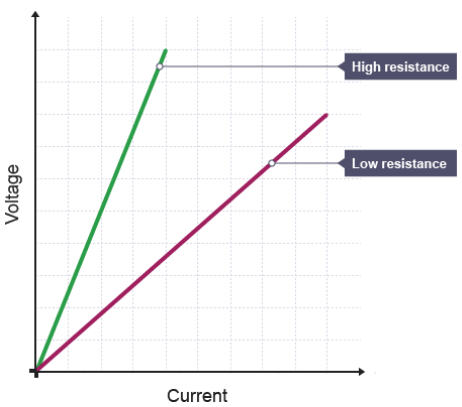
\includegraphics[width=0.7\textwidth]{img/VI_Curve.png}
    \caption{A Voltage vs Current plot. The slope represents resistance.}
    \label{fig:VI_Resistor}
\end{figure}
\\
Voltage, Resistance, and Current are related through the following equation: \\

\begin{center}
    Voltage = Current (I) $\times$ Resistance (R)
\end{center}
$$
V=IR
$$

This equation is known as \textbf{Ohm's Law}.

\section{Electrical Components}
\subsection{Resistor}
Resistors are used to reduce current and/or drop voltage.\\

\begin{figure}[h]
    \centering
    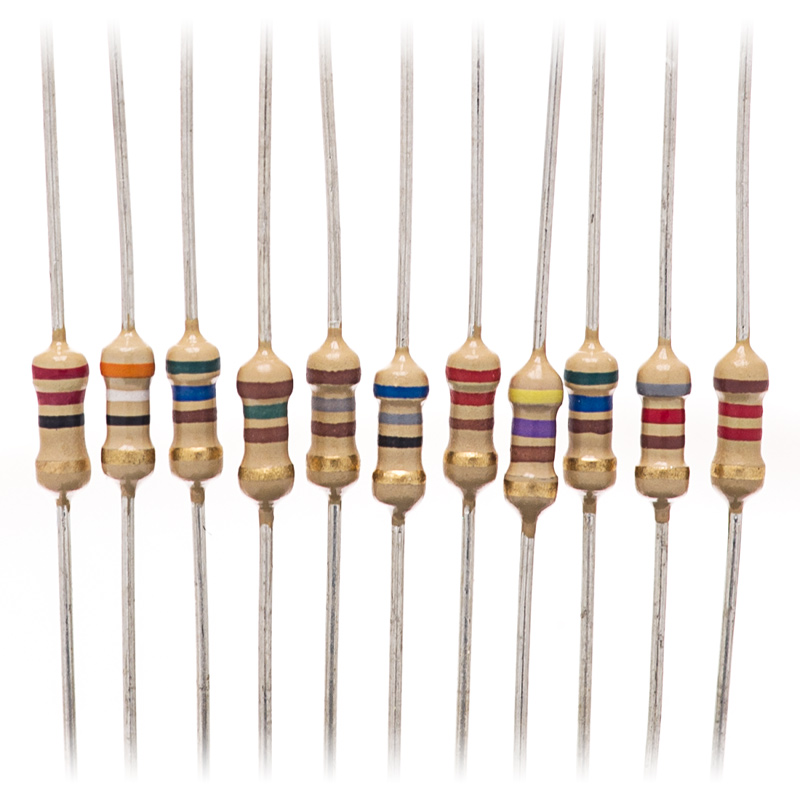
\includegraphics[width=0.5\textwidth]{img/resistors-thru-hole.jpg}
    \caption{Through-hole resistors come with different resistance values identified by the colored bands}
    \label{fig:res-thru}
\end{figure}

A \textbf{resistor} is a two-terminal \textbf{passive} (requires no external energy to operate) component that \textbf{implements electrical resistance} between the two terminals. Resistors are used to reduce current flow, adjust signal levels, divide voltage, etc.

The power dissipated by a resistor is calculated by multiplying voltage and current, $P =V \times I$, this may further expand to $P =V^{2}/R$ and $P= I^2R$. The first equation applies to the power dissipation of all electrical components, while the other two are for the case of resistors.

\begin{figure}[h]
    \centering
    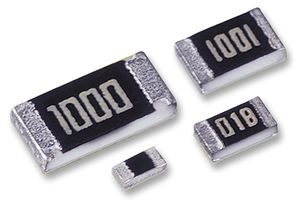
\includegraphics[width=0.5\textwidth]{img/resistors-smd.jpg}
    \caption{Surface mount resistors are normally used when designing PCBs}
    \label{fig:res-smd}
\end{figure}

Tip: The resistance of a wire is calculated with the formula R=pl/A (p=resistivity of the material, l=length of the wire, A=cross sectional area of the wire).


\subsection{Capacitor}

In short, capacitors store energy. \\
\begin{figure} [h]
    \centering
    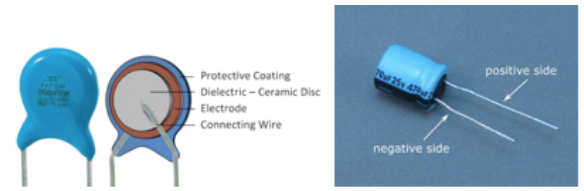
\includegraphics[width=0.9\textwidth]{img/Capacitors.png}
    \caption{Ceramic (left) and electrolytic capacitor (right).}
    \label{fig:capacitor}
\end{figure}

A \textbf{capacitor} is a \textbf{passive} two-terminal component that \textbf{stores energy in an electric field}. The larger the capacitance (which is noted as C), the more energy a capacitor can store and the longer it takes to charge and discharge.\\


There are primarily two kinds of capacitors: ceramic and electrolytic. In our scope of application, we need to know that electrolytic capacitors easily obtain high capacitance values with low cost and electrolytic ones are usually much larger compared to ceramics, rendering most capacitors on Printed Circuit Board (PCBs) to be ceramic. Electrolytic capacitors have polarity or a direction they must be in, in circuits. \\

Capacitors act as energy sources when discharging, so they’re often placed in parallel with voltage sources to maintain voltage levels during sudden load changes to prevent spikes. This application is known as “decoupling capacitance.”


\subsection{Inductor}

In short, an inductor limits current.
An \textbf{inductor}, also known as a coil, is a \textbf{passive} two-terminal component that stores energy in a \textbf{magnetic field}. An inductor, which has inductance noted as L, can help smooth sudden current spikes in the circuit as it stores current temporarily. Thus, they are commonly placed in series with power supplies. \\

Unlike a Capacitor which opposes a change of voltage across their plates, an inductor opposes the rate of change of current flowing through it due to the build up of self-induced energy within its magnetic field. In other words, inductors resist or oppose changes of current but will easily pass a constant current.\\

Inductors are also a primary component in electromechanical actuators such as relays (switches that use electromagnets), solenoids (values that use electromagnets), and motors (rotating devices that use electromagnets). 

\subsection{Diode}

In short, a diode allows current flow in one direction.\\

A \textbf{diode} is a two-terminal \textbf{passive} component that conducts current primarily in \textbf{one direction}. It ideally has zero resistance in one direction and infinite resistance in the other. In order for the diode to start operating in forward-bias mode, there has to be a threshold voltage across the diode (typically 0.7V). After this the diode will conduct electricity freely. \\

A common diode is the \textbf{Light Emitting Diode (LED)} that \textbf{emits light} when current passes through it. When designing an LED circuit, one must consider the maximum current the diode can handle and add a resistor if needed, or the LED could burn up from too much current. Below is an example of an LED circuit.

\begin{figure} [h]
    \centering
    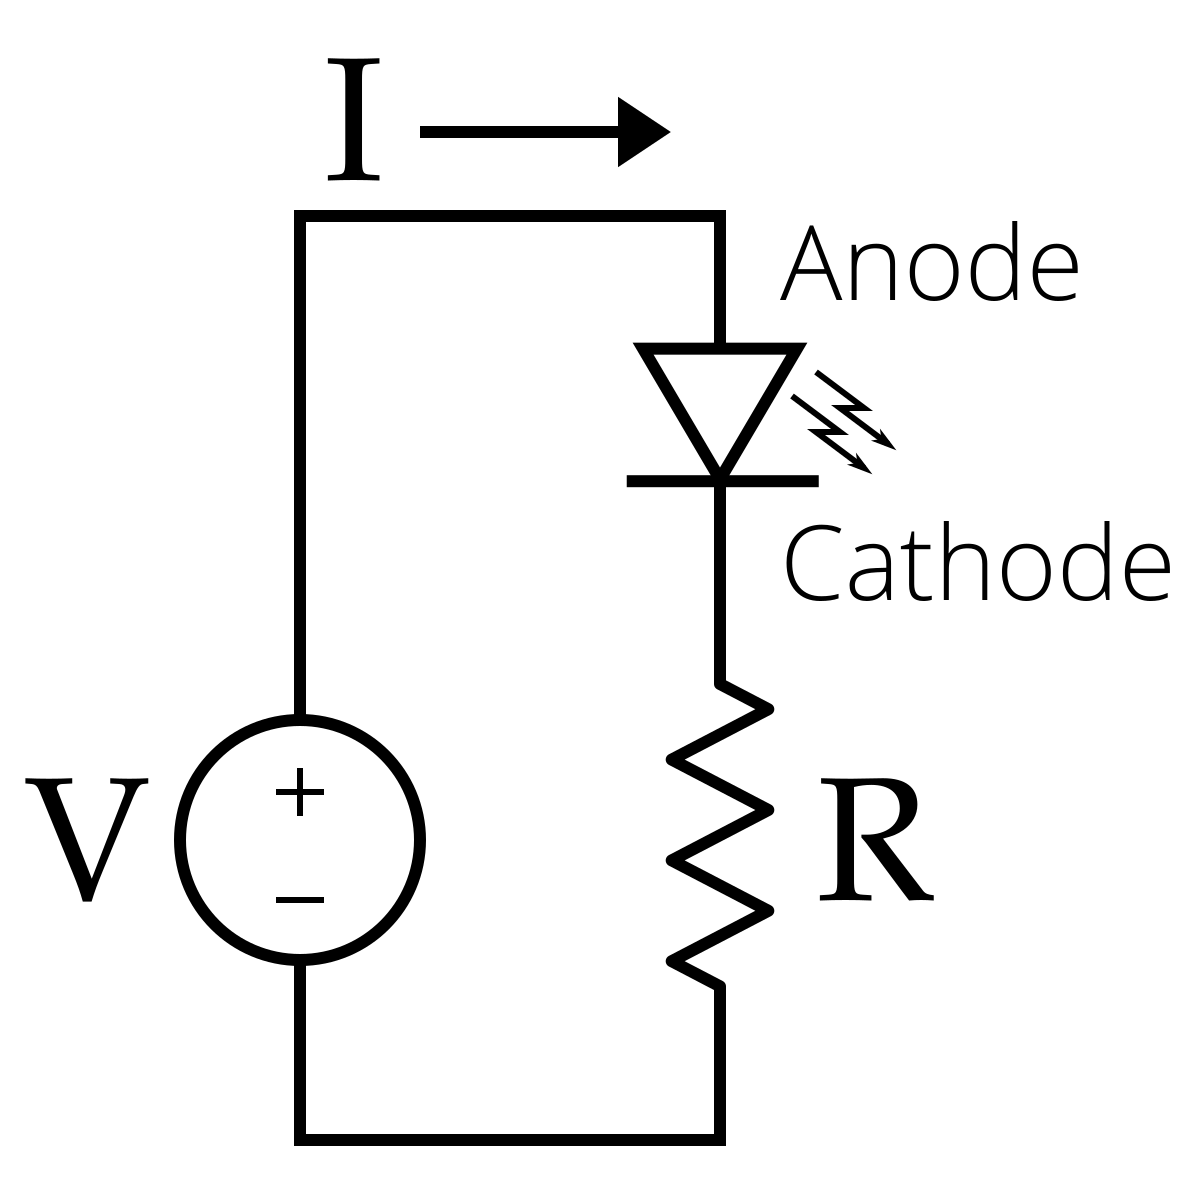
\includegraphics[width=0.5\textwidth]{img/LED_Circuit.png}
    \caption{LED Circuit.}
    \label{fig:LED_ckt}
\end{figure}

The value of R depends on the voltage applied and the type of LED and can be found from Ohm’s Law. \\

Diodes have many applications for reverse polarity protection (preventing current from flowing if the circuit is plugged in backwards) and voltage source protection (preventing current from flowing from one source to another). LEDs are used for indication and signaling of power levels, statuses, or faults. \\

Most diodes have a maximum \textbf{reverse voltage}: the breakdown voltage. Any higher than this voltage, and the diode will break down unless it is a \textbf{zener diode}, specifically designed to be reversible.


\subsection{Transistor}

In short, transistors are simple \textbf{electronic switches}. \\

There are primarily two types of transistors: Bipolar Junction Transistors (BJTs) and Metal Oxide-Semiconductor Field-Effect Transistors (MOSFETs). 

They typically have three terminals, the base or gate being the ‘controller’, and the other two being the collector or source and emitter or drain. There exist two types of BJT: NPN and PNP. NPN is normally OFF and conducts current when there is positive voltage at its base. PNP works in the exact opposite way, it is normally ON and conducts when there is zero voltage at its base. nFET and pFET MOSFETS work in a similar fashion to NPN and PNP respectively. Transistors are used to switch on other parts of the circuit.

\begin{figure} [h]
    \centering
    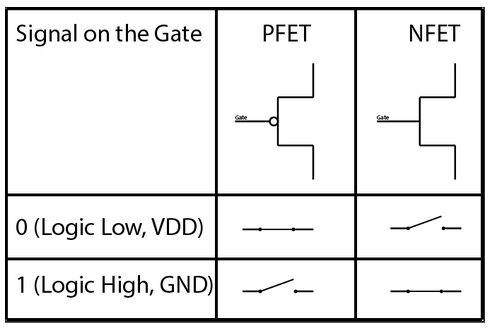
\includegraphics[width=0.7\textwidth]{img/TransistorSignal.png}
    \caption{Function of transistors based on gate logic levels}
    \label{fig:TranSignal}
\end{figure}

VDD (Voltage Drain Drain) is the power source of the system, or the ON voltage. GND is “the reference point in an electrical circuit from which voltages are measured” or the 0 voltage. For our applications, 3.3V or 5V are usually the logical operating levels of printed circuit boards with 12V or 24V are usually the voltage level that power the robot. 
Never directly connect 5V directly to 0V, as this is called a short circuit. 

\begin{figure} [h]
    \centering
    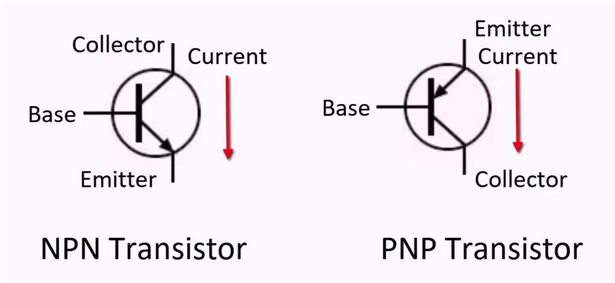
\includegraphics[width=0.7\textwidth]{img/TransistorCurrent.png}
    \caption{Transistor terminals and direction of current flow}
    \label{fig:TranCurr}
\end{figure}

\subsection{Fuse}

A \textbf{fuse} is a component that is designed to fail when there is \textbf{too much current} passing through it. When placed in series with your circuit, it is a safety device as it prevents over current.

Blown fuses alert you that there’s excessive current, implying either: 
\begin{enumerate}
    \item A component is broken or operating in an unsafe region
    \item The circuit must be redesigned taking into account maximum ratings
\end{enumerate}

\section{Circuit Analysis}

A circuit with components in \textbf{series} has all of its components on the same “path” whereas a circuit with its components in \textbf{parallel} has all of its components on different “paths.” 

\begin{figure} [h]
    \centering
    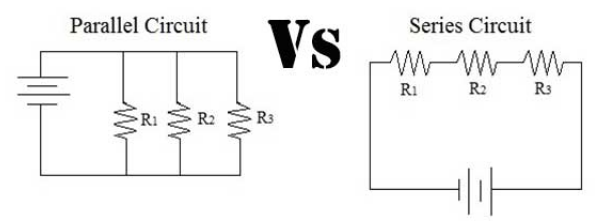
\includegraphics[width=\textwidth]{img/ParallelSeries.png}
    \caption{Example of resistors in parallel or series}
    \label{fig:ParallelSeries}
\end{figure}

\subsection{Series Circuit Component Formulas}

\begin{gather*}
R_{total} = R_{1} + R_{2} + R_{3} + \dots + R_{i} \\
\frac{1}{C_{total}} = \frac{1}{C_{1}} +  \frac{1}{C_{2}} + \frac{1}{C_{3}} + \dots + \frac{1}{C_{i}} \\
C_{total} = \frac{1}{\sum_{i} \sfrac{1}{C_{i}}} \\
L_{total} = L_{1} + L_{2} + L_{3} + \dots + L_{i}
\end{gather*}

\subsection{Parallel Circuit Component Formulas}

\begin{gather*}
\frac{1}{R_{total}} = \frac{1}{R_{1}} +  \frac{1}{R_{2}} + \frac{1}{R_{3}} + \dots + \frac{1}{R_{i}} \\
R_{total} = \frac{1}{\sum_{i} \sfrac{1}{R_{i}}} \\
C_{total} = C_{1} + C_{2} + C_{3} + \dots + C_{i} \\
\frac{1}{L_{total}} = \frac{1}{L_{1}} +  \frac{1}{L_{2}} + \frac{1}{L_{3}} + \dots + \frac{1}{L_{i}} \\
L_{total} = \frac{1}{\sum_{i} \sfrac{1}{L_{i}}} \\
\end{gather*}

\subsection{Further Reading}
\noindent \href{https://learn.sparkfun.com/tutorials/capacitors/introduction}{Capacitors - learn.sparkfun.com} \\
\href{https://www.allaboutcircuits.com/technical-articles/characteristics-of-the-ideal-diode/}{Characteristics of the Ideal Silicon Diode - Technical Articles}

\section{Circuit Basics}

\subsection{Kirchoff's Laws}
Kirchhoff's Current Law is that the sum of current flowing into a node (or a junction) must be equal to the sum of current flowing out of it.
Kirchhoff’s Voltage Law is that the algebraic sum of the voltage (potential) differences in any closed circuit must equal zero.

\begin{figure} [h]
    \centering
    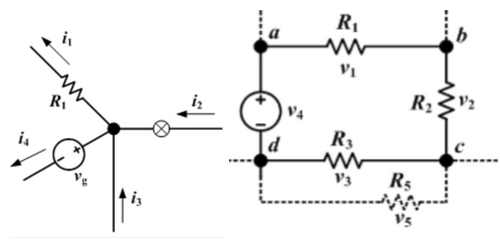
\includegraphics[width=0.8\textwidth]{img/Kirchoff.png}
    \caption{Kirchoff's junction and loop laws}
    \label{fig:Kirchoff}
\end{figure}

As defined by Kirchhoff’s law, in the left diagram $i_{2} + i_{3} = i_{1} + i_{4}$; in the right figure,
$v_{1} + v_{2} + v_{3} + v_{4} = 0$

\subsection{Breadboard}
In short, a \textbf{breadboard} is a device allowing you to \textbf{prototype} circuits. \\

It offers the ability to let you connect circuits by directly plugging them into it, saving you the effort of making a PCB.

\begin{figure} [h]
    \centering
    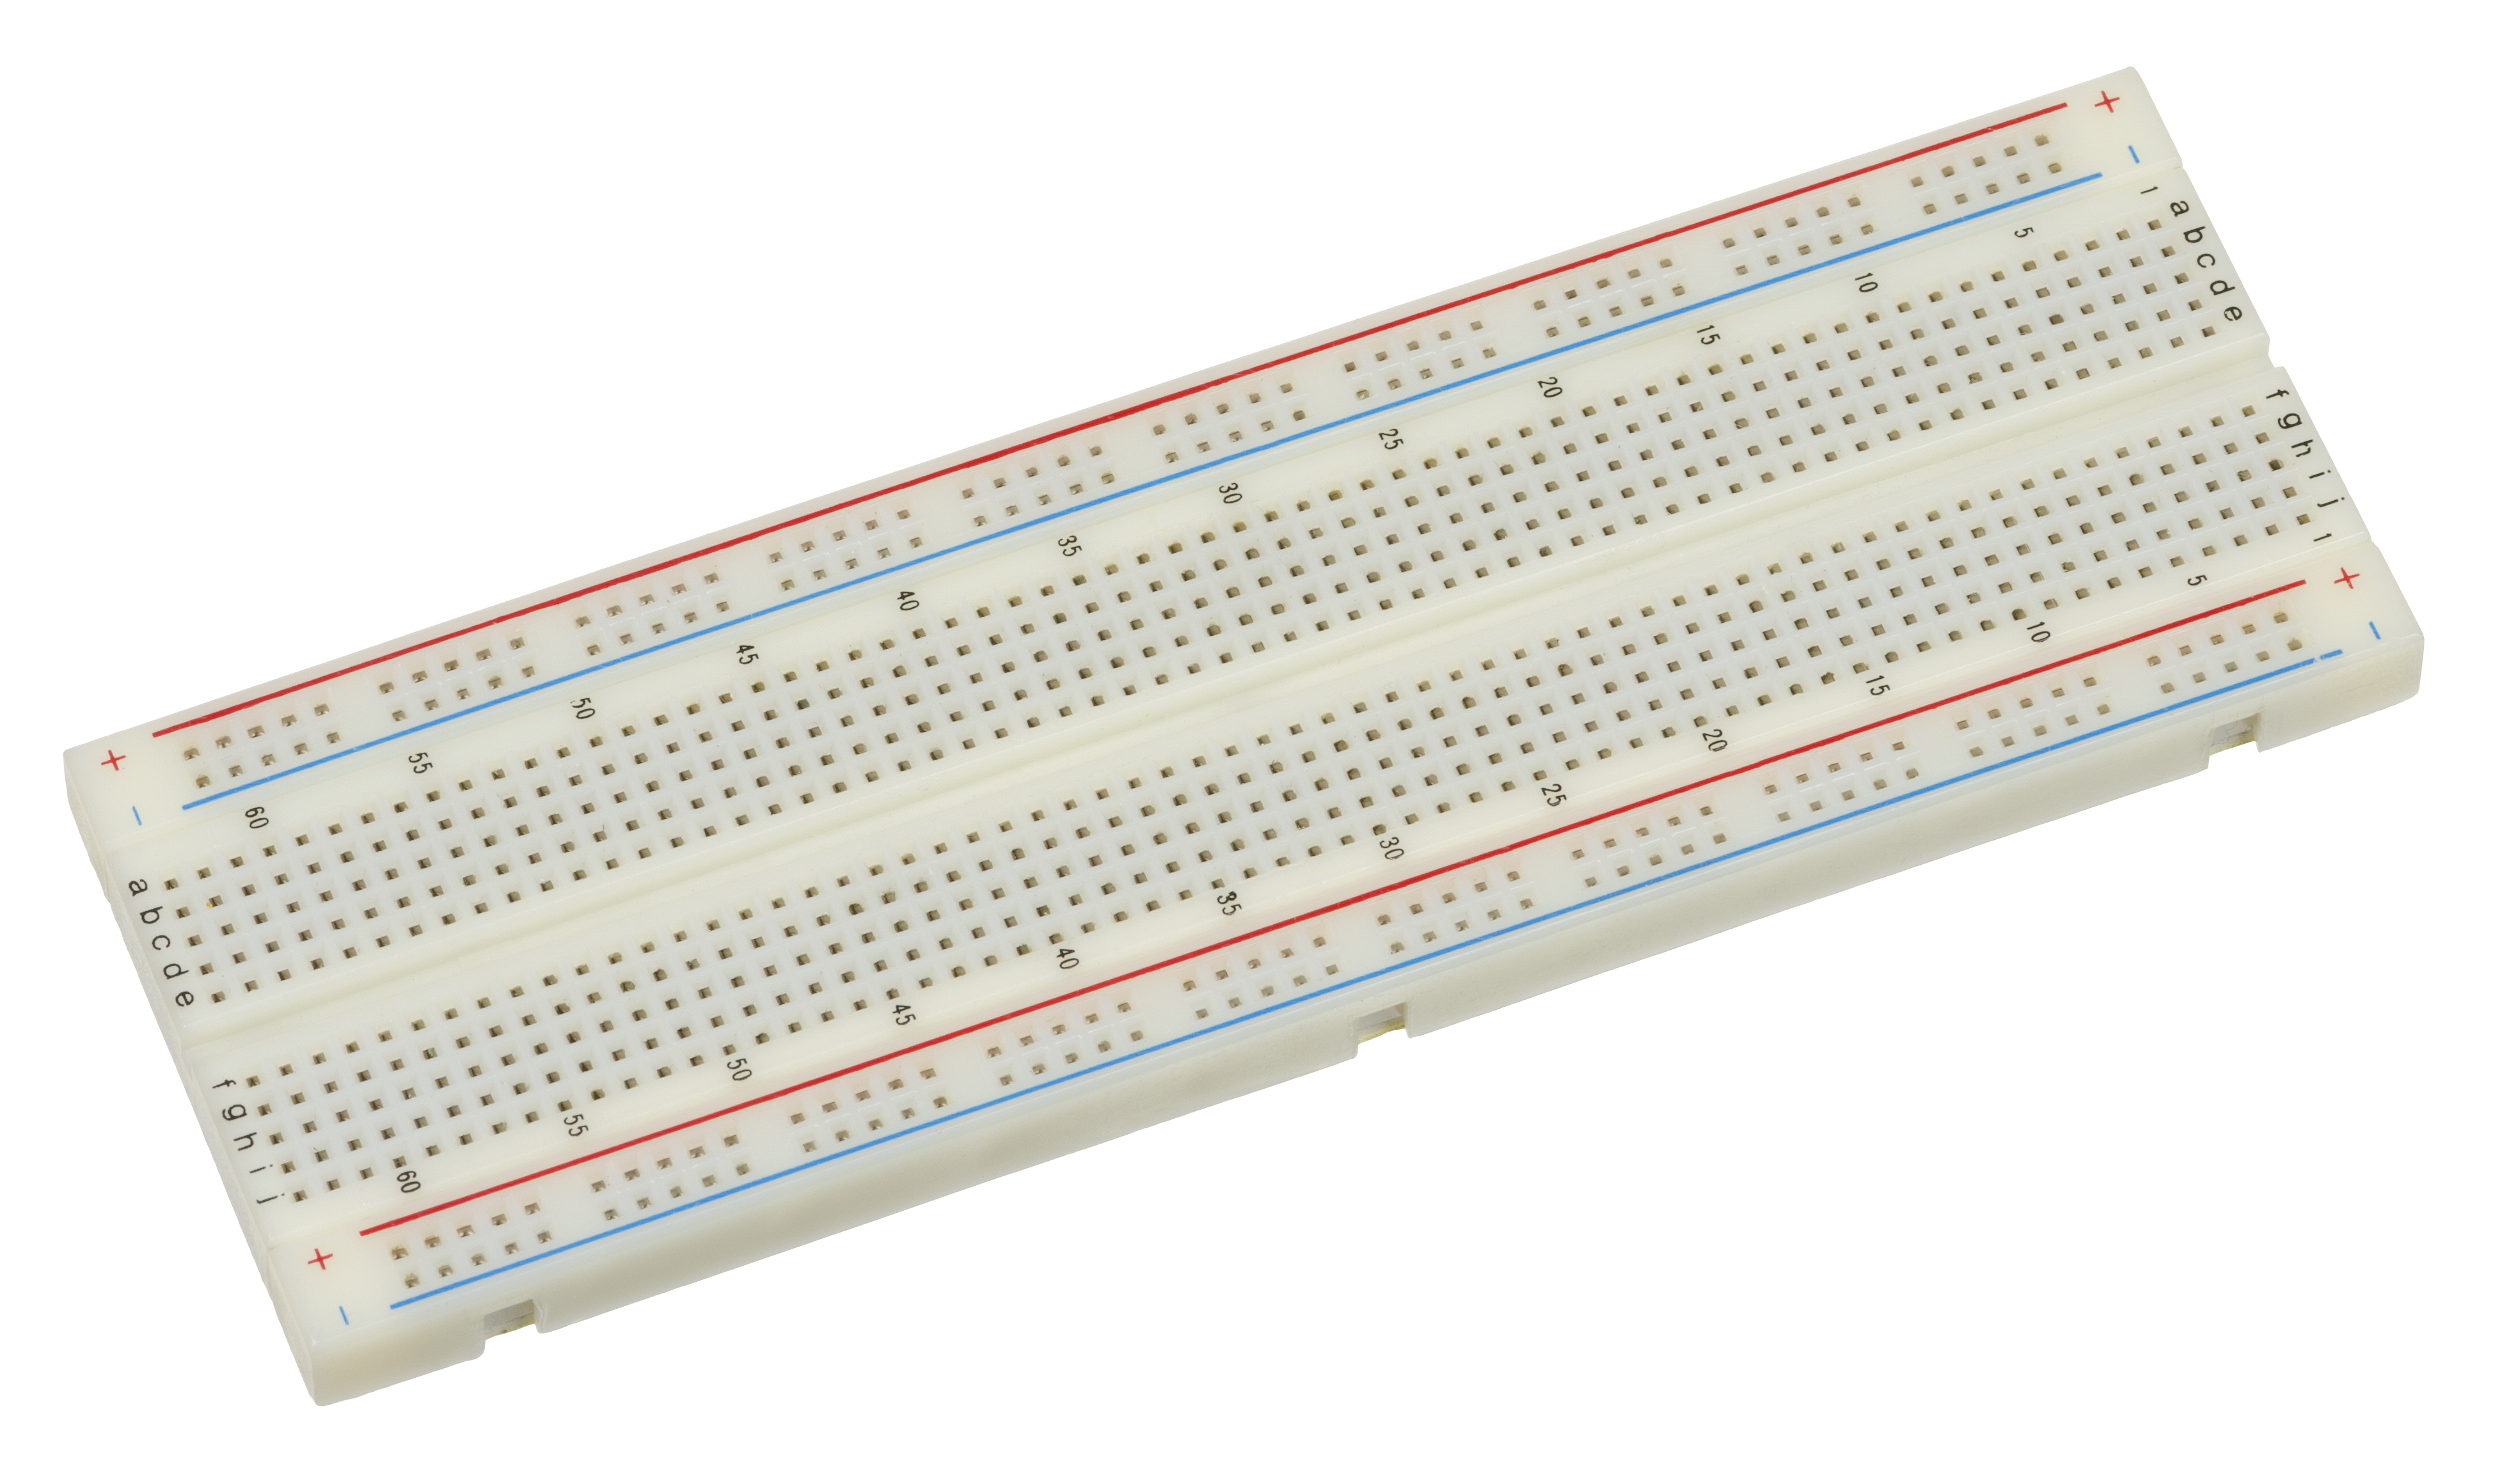
\includegraphics[width=0.6\textwidth]{img/Electronics-White-Breadboard.jpg}
    \caption{A Breadboard}
    \label{fig:breadboard}
\end{figure}

\pagebreak

\section{Common Circuit Designs}

\subsection{Voltage Divider}
The goal of a voltage divider is to reduce the voltage in your circuit. The input voltage is distributed among the two resistors shown below, with the output voltage emerging from the connection between the resistors and the second resistor being connected to ground.

\begin{figure}[h]
    \centering
    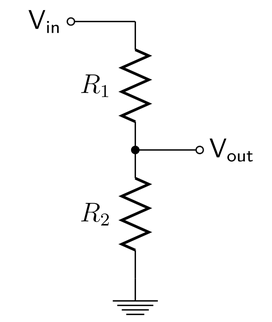
\includegraphics[width=0.4\textwidth]{img/Voltage_Div.png}
    \caption{A voltage divider circuit.}
    \label{fig:VoltageDiv}
\end{figure}

To calculate the output voltage of the circuit, the following formula can be used. 
$$
V_{out} = \frac{R_{2}}{R_{1} + R_{2}}
$$

\subsection{High/Low Side Switch}
High/low side switches two different ways to configure a circuit. A low side switch connects the load (the portion of the circuit that consumes power, shown as a box below) to ground using an N-type MOSFET. On the other hand, a high side switch connects power to the load using a P-type MOSFET.

\begin{figure} [h]
    \centering
    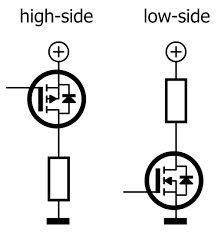
\includegraphics[width=0.4\textwidth]{img/high_low_switch.png}
    \caption{A high-side switch, using a PFET, and a low-side switch, using an NFET }
    \label{fig:my_label}
\end{figure}

So how do you decide which one to use? In most scenarios, a low-side switch would work. Low-side switches are especially useful when dealing with high voltage circuits. If you are delivering power to an entire circuit or a voltage-sensitive device, a high-side switch may be applicable.

\subsection{Pull Up/Pull Down Resistor}
In a digital logic circuit, there must only be a Low state (GND or 0) or a High state (Vcc or 1) and a Pull-Up and Pull-Down resistor ensures this. 

\begin{figure} [h]
    \centering
    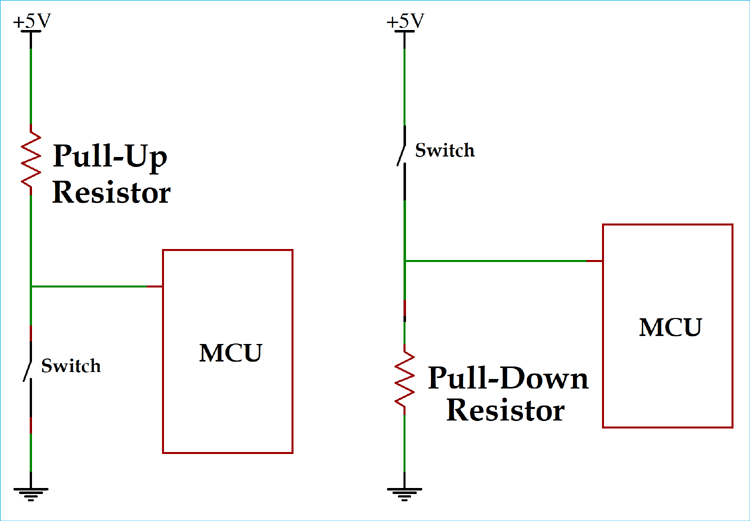
\includegraphics[width = 0.5\textwidth]{img/Pull-up-and-Pull-down-Resistor.png}
    \caption{Pull up and pull down resistors on a Microcontroller's input pins}
    \label{fig:PullUpDown}
\end{figure}

In figure \ref{fig:PullUpDown} for a Pull-Up Resistor, we see a +5V source, resistor, ground, switch, and an input to a microcontroller. When the switch is opened, the 5V source provides an input current to the microcontroller which is a logic of 1. When the switch is closed, the resistor causes a small amount of current to flow to ground thus making the microcontroller input a logic of 0. 

A similar process applies to a Pull-Down Resistor as well. When the switch is closed in this circuit, the input of the microcontroller with get 5V or a logic of 1. When it is open, it receives a logic 0.

Note, if we didn’t have the resistor in these circuits, the 5V source would be directly connected to ground without any resistance and this will end up shorting the circuit which we never want to do.

\section{Decoupling/Bypass Capacitor}
In short, a decoupling capacitor's job is to suppress high-frequency noise in power supply signals.

Many electronics use decoupling capacitors to make sure the chip is not subjected to any big dips or spikes in voltage.
Decoupling capacitors are used between the power source and ground as shown in the figure below. It is quite common to use more than one capacitor to bypass the power supply. 

\begin{figure} [h]
    \centering
    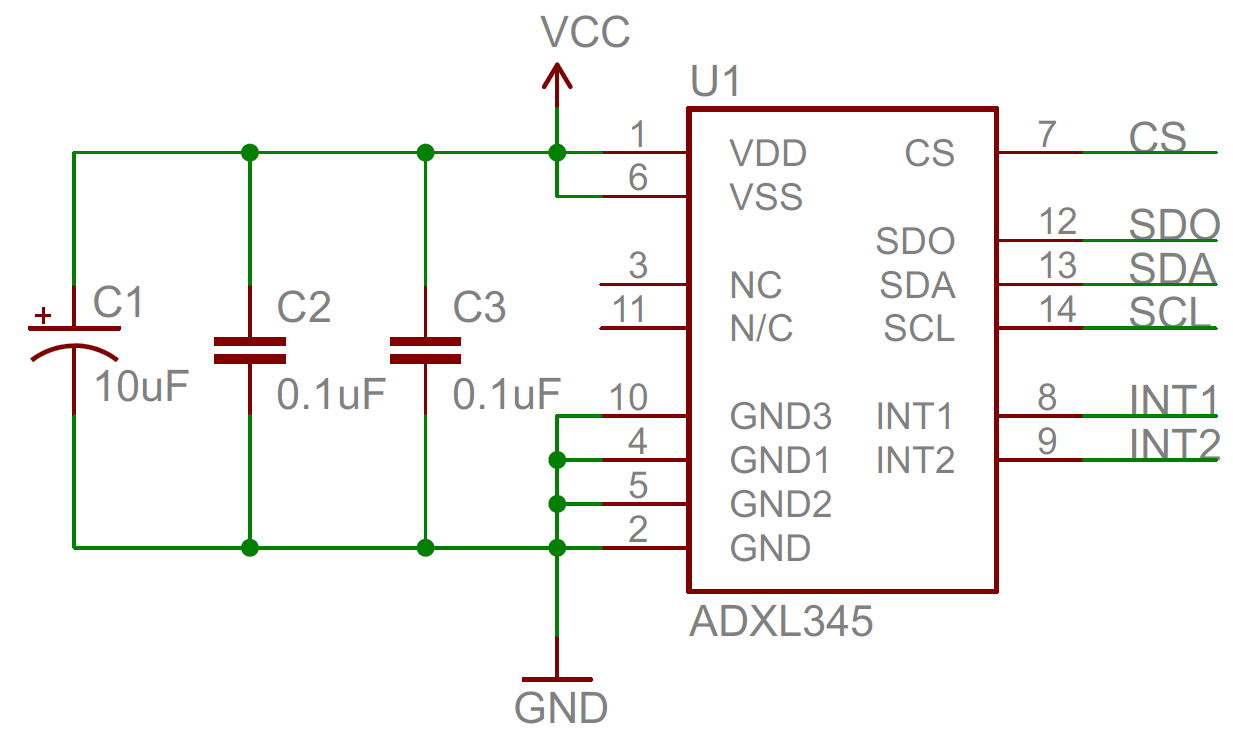
\includegraphics[width=0.7\textwidth]{img/DecouplingCap.png}
    \caption{Decouling Capacitors used for an IC. Source: \href{https://learn.sparkfun.com/tutorials/capacitors/application-examples}{Sparkfun.com}}
    \label{fig:DecouplingCap}
\end{figure}


\end{document}
